\documentclass[a4paper,12pt]{article}
\usepackage[pdftex]{graphicx}


\begin{document}


\begin{titlepage}
\begin{center}
\textsc{\LARGE Assignment 7} \\[1.5cm]
\textsc{\large Stochastic PetriNets} \\[2.5cm]
\textsc{Harshit Kumar Gupta} \\
\textsc{Entry No. 2013EET2369} \\[2.5cm]
\begin{center}
 
\includegraphics{iitd.png}
 % iitd.jpg: 200x204 pixel, 96dpi, 5.29x5.40 cm, bb=0 0 150 153
\end{center}

\textsc{Computer Technology} \\
\textsc{Department of electrical Engineering} \\
\textsc{Indian Institute of Technology Delhi} \\
\vfill
\textsc{\today} \\
\end{center}


\end{titlepage}

\tableofcontents

\newpage

\section{Problem Statement :}
                             Simulate the given Model in the paper(PFA) in Sharpe and obtain the results and also plot the graph b/w
                  \begin{itemize}
                             \item arrival rate v/s throwput
                             \item virtual load v/s throwput
                   \end{itemize}

\begin{center}
 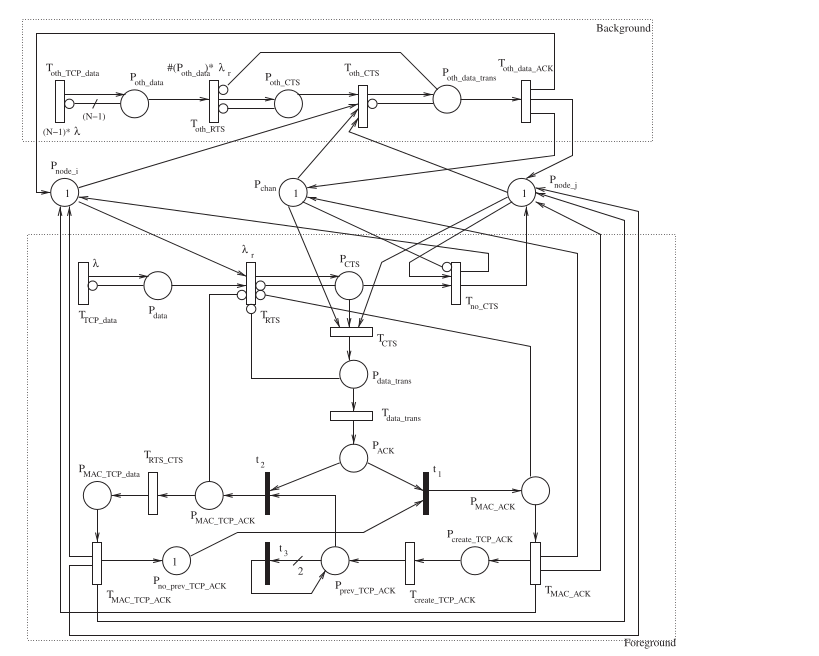
\includegraphics{file.png}
 % file.png: 396x722 pixel, 72dpi, 13.97x25.47 cm, bb=0 0 396 722
\end{center}

 \newpage     
      
\section{Theory :}

\subsection{Sharpe GUI :}

The SHARPE GUI implements eight interchangeable modeling description
techniques for reliability engineering: fault trees, Markov chains, reliability
block diagrams, reliability graphs, generalized stochastic Petri nets,
product queuing networks, multi-chain product form queuing networks
and task graphs. future, all the modeling description techniques contained
in SHARPE will be available in the GUI (phase mission, multi-components
fault trees, semi-Markov chains).
\begin{center}
 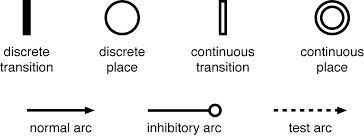
\includegraphics{petrisym.jpeg}
 % patri1.png: 211x239 pixel, 72dpi, 7.44x8.43 cm, bb=0 0 211 239
\end{center}


\subsection{Stochastic  PetriNets :}

Petri Nets (PN) are a graphical tool for the formal description of the flow of activities in
complex systems. With respect to other more popular techniques of graphical system rep-
resentation (like block diagrams or logical trees), PN are particularly suited to represent in
a natural way logical interactions among parts or activities in a system. Typical situations
that can be modelled by PN are synchronization, sequentiality, concurrency and conflict.

A petrinet is represented as a quintuple (P, T, I, O, M ), where: \\
\begin{itemize}
  \item  P = {p1 , p2 , . . . , pnp } is the set of np places (drawn as circles in the graphical repre-
sentation)
  \item T = {t1 , t2 , . . . , tnt } is the set of nt transitions (drawn as bars)
  \item I is the transition input relation and is represented by means of arcs directed from
places to transitions
  \item O is the transition output relation and is represented by means of arcs directed from
transitions to places
  \item M = {m1 , m2 , . . . , mnp } is the marking. The generic entry mi is the number of
tokens (drawn as black dots) in place pi in marking M 
\end{itemize}
 \newpage
\section{Approach :}
\begin{itemize}
\item There are two main parts of this model.
\item The upper part of the model (the small dashed rectangle) represents the background traffic activity  \\ 
      generated by N ambient nodes in the ad hoc network, i.e. it captures the cumulative behavior of all \\
      the other stations. 
\item The lower part of the model (the large dashed rectangle) represents the foreground traffic activity between two \\
      representative nodes i and j in the network, i.e. it captures the behavior of the reference station
      in \\ detail. The three circles in the gap between the two rectangles represent the TCP sender i (on
      the left), the TCP receiver j (on the right), and the shared wireless channel (in the middle). The
      places, timed transitions, and immediate transitions.
\item the SRN model assumes exponentially distributed firing times for all the timed transitions, although \\
      some events in the SRN model might be deterministic rather than random.
\item This is represented by the firing of the timed transition TRTS .
\item The firing time of TRTS is exponentially distributed with parameter r .
\end{itemize}
\newpage
\section {Specification and Assumpation :}
 Specification and assumption are :
 \begin{itemize}
 \subsection{Specification :}
\item we develop the SRN model for the original IEEE 802.11 MAC protocol with
       RTS/CTS mechanism.
\item This model assumes a single shared channel for operation.
\item This implementation is based on SHARP TOOLS implementation and Stochastic  PetriNets knowledge.
\item Deals with the simulation of IEEE 802.11 mac protocol with RTS/CTS mechanism.
\subsection {Assumption :}
\item The SRN model assumes exponentially distributed firing times for all the timed transitions, \\ although some events in the SRN model might be deterministic 
\item The firing time of TTCP data is exponentially distributed with parameter .
\item It is sufficient to model the DCF operations of the HoL packets at all stations.
\item Arrival rate propotional to tha packet size.
\item Virtual load will be propotional to the square of the arrival rate.
\end{itemize}

\newpage

\section {Working  :}
The upper part of the model (the small dashed rectangle) represents the
background traffic activity generated by N ambient nodes in the ad hoc net-
work, i.e. it captures the cumulative behavior of all the other stations. The
lower part of the model (the large dashed rectangle) represents the foreground
traffic activity (i.e. the movement of TCP data packets and TCP acknowl-
edgements) between two representative nodes i and j in the network, i.e. it
captures the behavior of the reference station in detail. The three circles in
the gap between the two rectangles represent the TCP sender i (on the left),
the TCP receiver j (on the right), and the shared wireless channel (in the
middle).

\section {Performance Measures  :}
Performance measures
Average system throughput
The average system throughput is given by :
 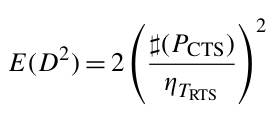
\includegraphics[]{formula.png}
Mean Delay
The delay of a packet is defined as the time spent by a packet in the system
until it is successfully transmitted (i.e. the packet is received correctly by
the destination station, and the corresponding ACK is received correctly by
the source station).
The delay can be calculated as follows
 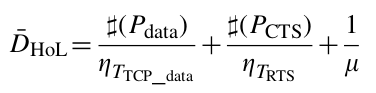
\includegraphics[scale=0.5]{formula2.png}
 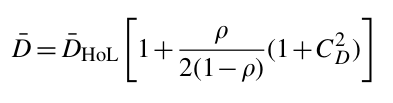
\includegraphics[scale=0.5]{formula3.png}
 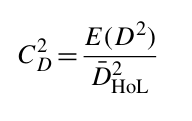
\includegraphics[scale=0.5]{formula4.png}
 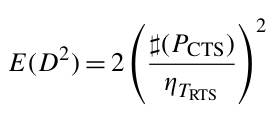
\includegraphics[scale=0.5]{formula5.png}
The mean delay obtained above is the mean delay suffered by any packet
in the system because all the stations are independent and behave identically.

%\section {Flow chart :}
%\begin{center}
 %\includegraphics[width=15 cm,height=13 cm]{Flow.png}
 % Flow.png: 375x635 pixel, 72dpi, 13.23x22.40 cm, bb=0 0 375 635
%\end{center}

\newpage

\section{Result :}
Here the graph is gentared for each scenario so the observation is shown blow .



The observed  Graph are :

\begin{center}
\subsection {lma v/s throwput :}
 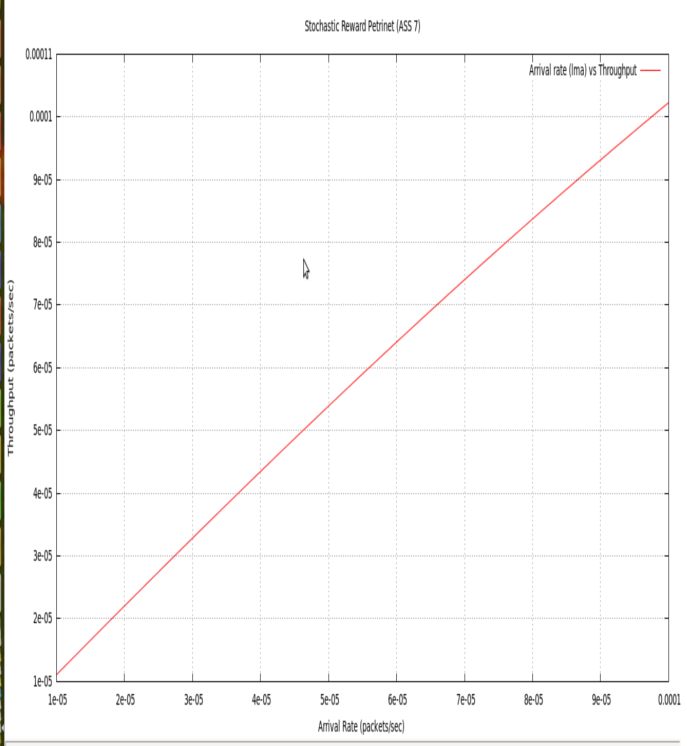
\includegraphics[width=15 cm,height=13 cm]{G1.png}
 % G1.png: 687x746 pixel, 72dpi, 24.24x26.32 cm, bb=0 0 687 746
\end{center}

\begin{center}
\subsection {virtual load v/s throwput :}
 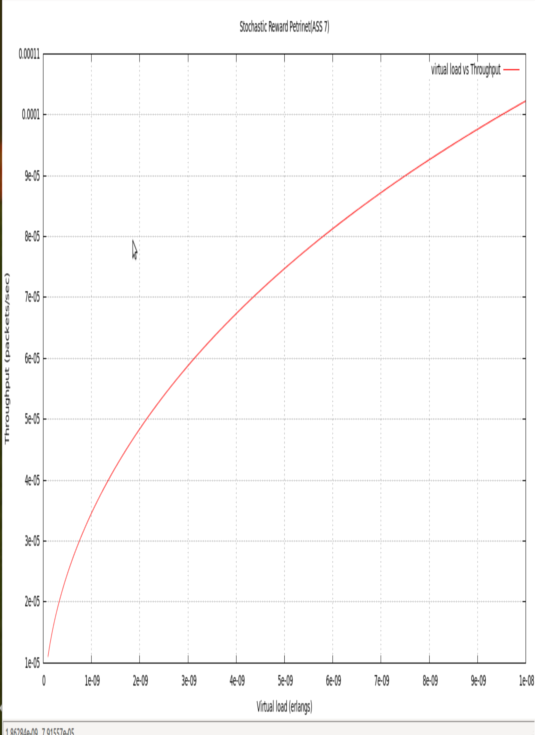
\includegraphics[width=15 cm,height=13 cm]{G2.png}
 % G2.png: 541x735 pixel, 72dpi, 19.09x25.93 cm, bb=0 0 541 735
\end{center}
\begin{center}
\subsection {Avg Throughput v/s Packet Size :}
 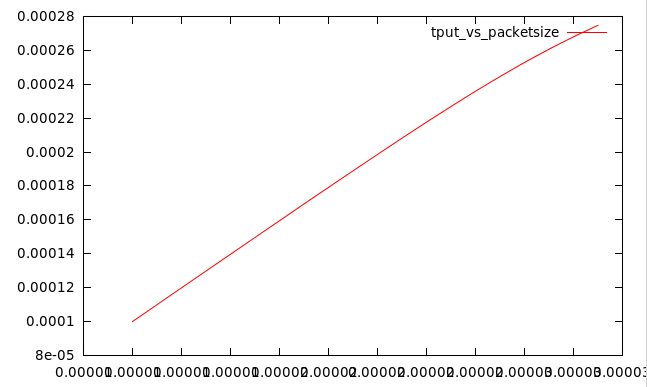
\includegraphics[width=15 cm,height=13 cm]{tput_packetsize.png}
 % G2.png: 541x735 pixel, 72dpi, 19.09x25.93 cm, bb=0 0 541 735
\end{center}
\begin{center}
\subsection {Avg Throughput v/s No Of NOdes :}
 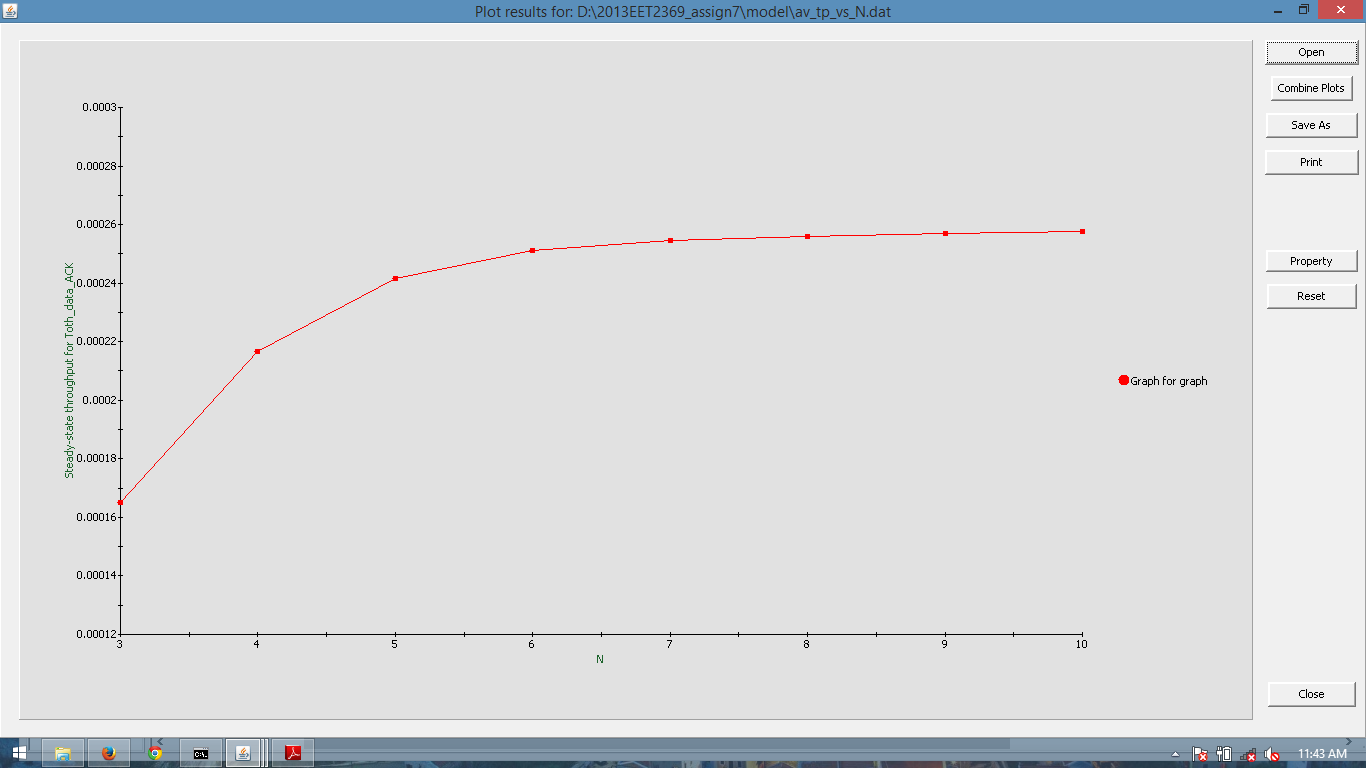
\includegraphics[width=15 cm,height=13 cm]{av_tp_vsN.png}
 % G2.png: 541x735 pixel, 72dpi, 19.09x25.93 cm, bb=0 0 541 735
\end{center}
\newpage
\section{Conclusion And Output :}

\begin{itemize}
  \item The given model has been modelled using SRN.
  \item The Graph is plotted b/w arrivalrate and throwput, and the second graph is plotted b/w virtual load and throwput.
  \item The difference b/w two graph is shown in graph .
\end{itemize}
 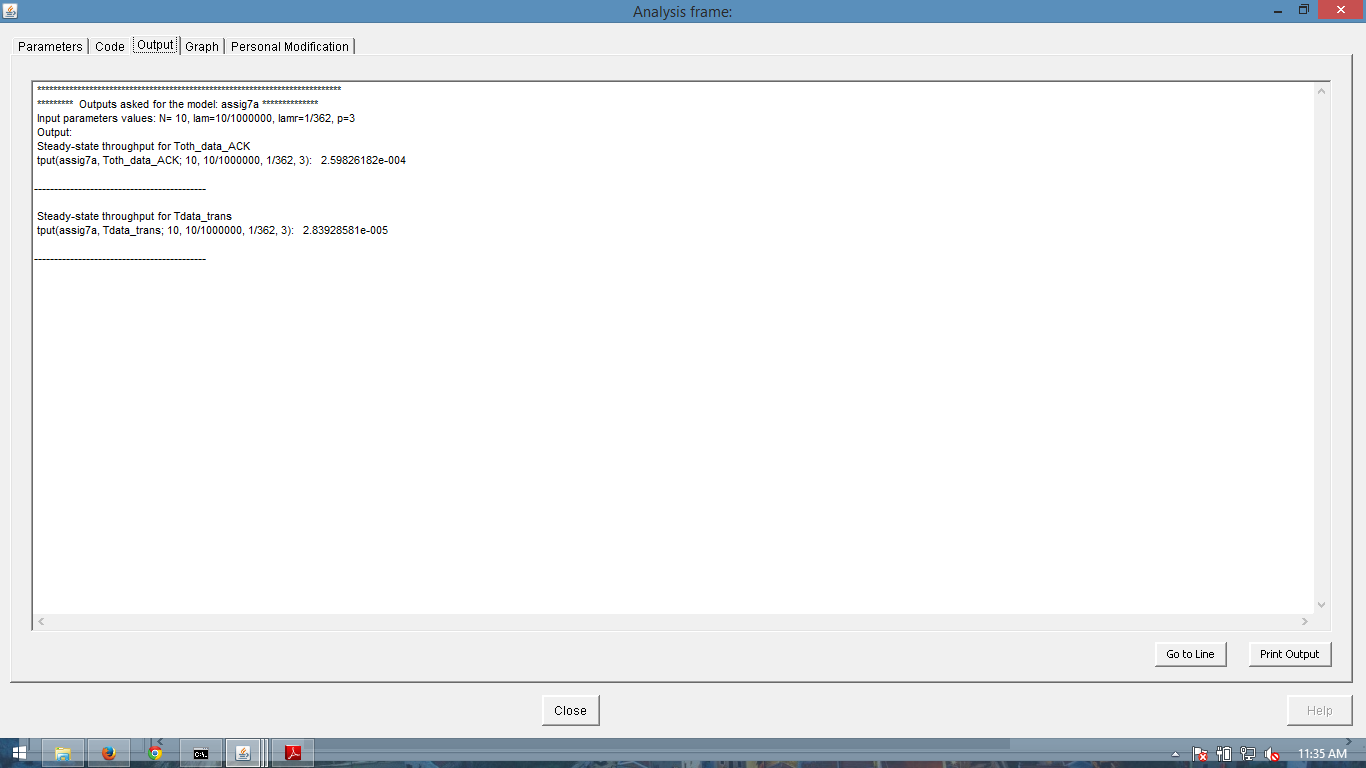
\includegraphics[width=15 cm,height=13 cm]{output1.png}
 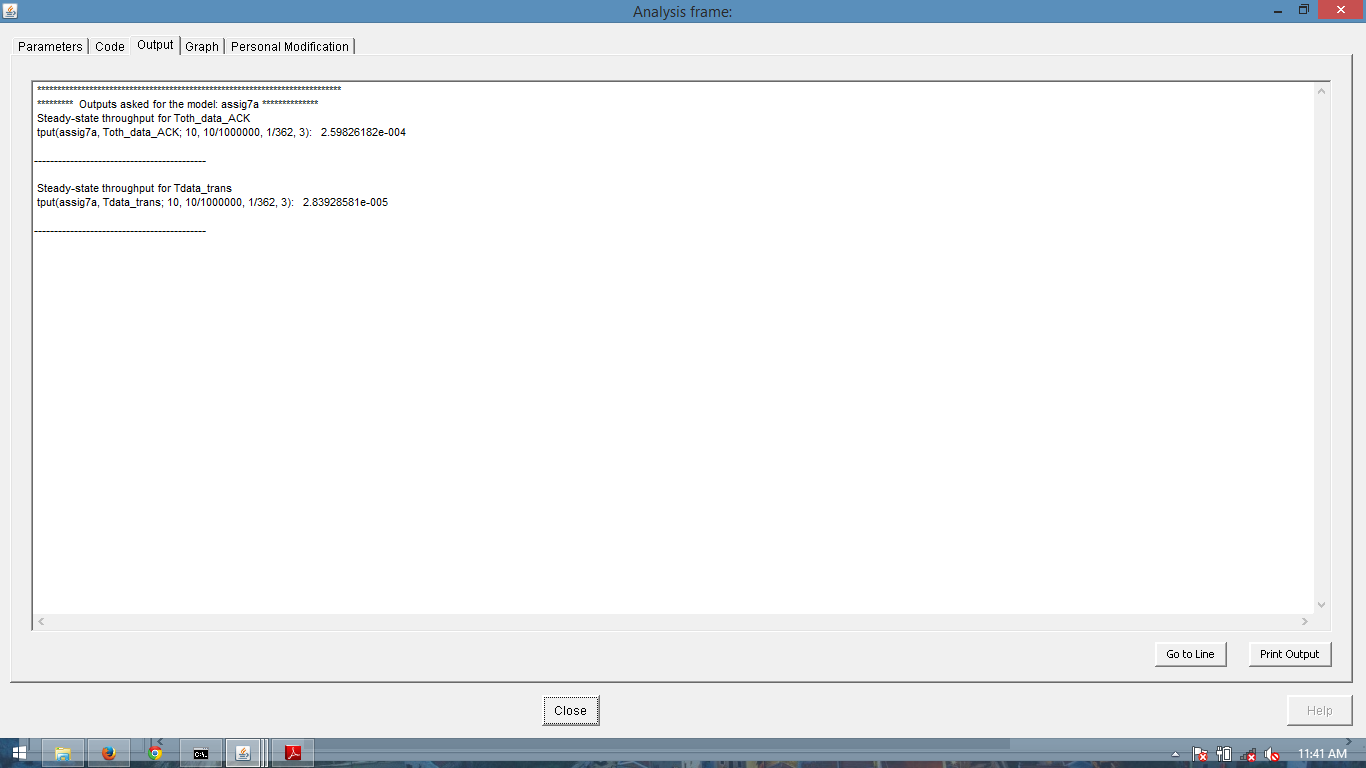
\includegraphics[width=15 cm,height=13 cm]{output2.png}



\end{document}
